\documentclass[../main.tex]{subfiles}
\graphicspath{{\subfix{../../images/}}}
\begin{document}

\chapter{Experimental Methods}\label{chap:methods}

\bigskip
\begin{quote}
    \emph{We have some idea as to the intricate design of the puppet and the puppet strings, but we lack insight into the mind of the puppeteer\cite{bizziHardScientificQuest2015}.}\\
    \raggedleft{--- Emilio Bizzi \& Robert Ajemian, 2015}
\end{quote}

\cleardoublepage%


\section{Methodological Aims}\label{sec:methods_aims}

\begin{itemize}
  \item Our goal is to explore EMG as a paradigm, particularly with a high degree of redundancy. Most tasks use a few muscles, we want to capture as much of the activity driving the hand as we can using surface EMG
  \item We're interested in the hand because, we argue (with others, mostly anthropologists), that along with language the hand is the most evolutionarily advanced \textit{thing} in the known universe! How we control it \textit{flexibly} is a huge open question, something we have yet to achieve \textit{in silico}
  \item We choose EMG because it is the ``raw'' signal directly from the brain, circumventing constraints and idiosyncrasies of joint kinematics\ldots (this needs more thought, what are these idiosyncrasies?). EMG gives us access directly to the physiology of the nervous system, rather than a proxy.
  \item We want to develop a task with:
  \begin{itemize}
    \item continuous action space--- not a discrete choice
    \item redundancy--- more input variables (e.g. muscles) than output (task-relevant) variables, and control over the redundant mapping between inputs and outputs\endnote{The concept of redundancy is common: in the human perception of color, we have a 3-dimensional plane of perception red, green, blue, while the space of physical colors is an infinite-dimensional spectrum. Thus, we can perceive some colors (e.g. yellow light vs. green+red light) with different spectra as identical, as they are identical when ``projected'' onto our perceptual plane (this is known as metamerism).}
    \item ``closed loop'' control-- subjects should interact with their virtual environment in real time
    \item development of a new skill, rather than adaptation of a known movement to a contingency (though this is blurry! ``Skill'' is not well defined. (Should we try to define it?))
    \item ``slow'' learning--- we want to track subjects' progress over many trials. If they learn too quickly, we may miss the subtleties of their progress. This requires us to titrate the difficulty of the task to a degree that makes the taska real challenge for subjects but is learnable. How we attempt to achieve this is explained in \Cref{sec:decoder_fitting}
    \item subjects' embodying, as much as possible, an infant-like state of ignorance within their bodies. They will understand the task intellectually (as its simple to explain the goal) but there is no ``trick'' to the task; it requires using your muscles in a new way
    \item the requirement that subjects use available, but uncommon, motor activation patterns. If the required patterns are commonly used in subjects' everyday life, the task may become a straightforward search and recall, as opposed to a building up of new motor solutions to the task goal
  \end{itemize}
  \item The questions our paradigm should allow us to access are:
  \begin{itemize}
    \item Do we learn ``from scratch'' or \textit{de novo}? Or do we reconfigure existing primitives?
    \item Do we uncover to task redundancy and use this to our advantage from the beginning of learning?
    \item What sequential decisions do subjects make in their choice of muscle activations?
  \end{itemize}
\end{itemize}


\begin{figure}[H]%[tph]
  \centering
  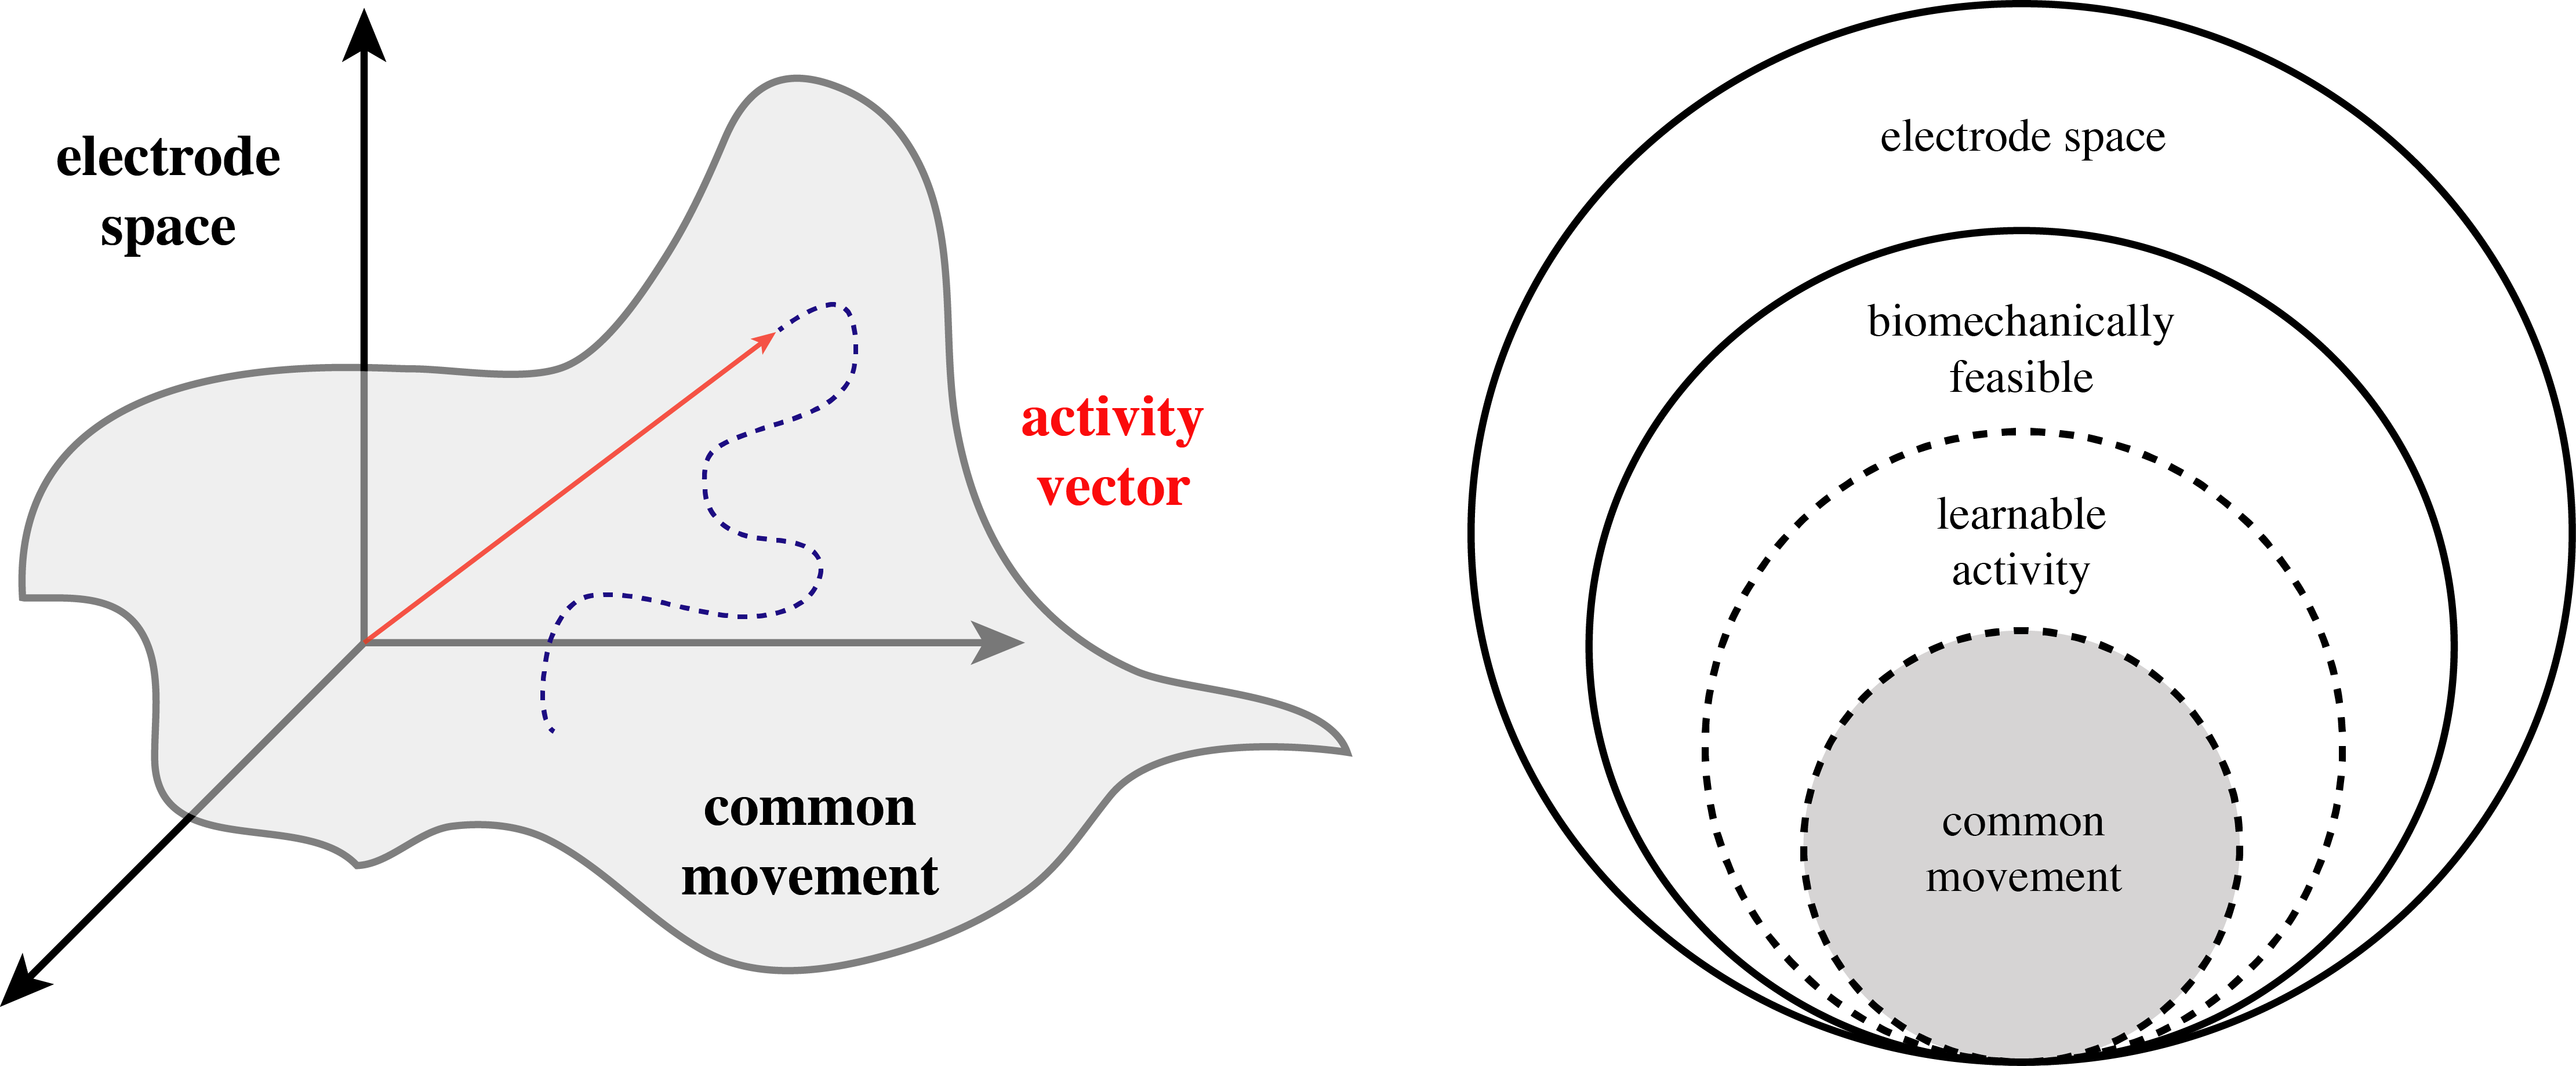
\includegraphics[width=1.0\textwidth]{methods/spaces.png}
  \caption[Geometry of the task]{PLACEHOLDER for a figure here or later which summarizes the EMG and task spaces and gives a visual intuition for the linear algebra}\label{fig:spaces}
\end{figure}


\section{Recording Setup}\label{sec:setup}

Hardware
\begin{itemize}
  \item The hardware was purpose-built for this experiment
  \item ``Sessantaquattro'' EMG amplifier acquired from OT Bioelettronica. This amplifier transmits data over WiFi, enabling more recording flexibility in terms of wiring and placement
  \item Custom electronic connection printed circuit board to connect the amplifier to 64 monopolar electrodes
  \item electrodes acquired from UniMed UK: 10mm Ag-AgCl cup reusable electrodes 
  \item conductive gel acquired from UniMed UK used: AC Cream
  \item reference electrode attached to subjects' ulnar styloid
  \item EMG signals are captured at 2kHz with 24-bit precision
  \item short segment of raw data is shown in \Cref{fig:raw_data}
  \item Several prototypes were made and tested for an electrode arrangement which permitted different size arms, was comfortable for the wearer, and ensured that electrodes remained in contact with the skin
  \item Final design was an elastic sleeve with the ability to ``snap'' connect electrodes to the sleeve to allow for different sized arms.
  \item The subject's arm is constrained in a foam-filled fixture to encourage isometric contractions. This enables the experiment to me more repeatable over subjects and decreases the likelihood of signal artefacts
  \item The subject's arm is encolsed within a metal frame to shield noise as well as remove the arm from the subject's field of view. See \Cref{fig:prototype_setup,fig:final_setup}
  \item 64 electrodes were attached to subjects' arms in a rectangular grid pattern, attempting to cover as much of the forearm musculature as possible \Cref{fig:muscle_map}
\end{itemize}

Software
\begin{itemize}
  \item Bonsai programming environment (C\# and Python) used for online data capture and presentation of visual feedback
  \item Python used for offline analyses
  \item All software is available upon request
  \item Raw EMG as recorded is shown in \Cref{fig:raw_data}
\end{itemize}

\begin{figure}[H]%[tph]
\centering
\includegraphics[width=1.0\textwidth]{methods/setup.pdf}
\caption[Experimental setup prototype]{(a) Graphic depicting the closed-loop EMG interface concept in a target task. The multidimensional EMG signal is transformed online through a mapping $F$ from EMG electrode space to a lower dimensional task space, creating an experimentally controllable redundancy problem for the subject. In experiments shown here the task space is two-dimensional, though the EMG interface can be extended to tasks with higher-dimensional inputs. The subject's arm and hand are constrained during the experiment to ensure isometric contractions. (b) First prototype of custom recording hardware consisting of four bands of eight electrodes each, and a spherical hand constraint. Our recordings are 64 channel monopolar recording with reference electrode at the wrist. (c) Example cup-style monopolar recording electrodes, 5mm in diameter. (d) Side view of the recording hardware. Also pictured is the arm restraint frame to ensure isometric contractions. The frame obscures the subject's arm from view and contains adjustable elbow and wrist rests. (d) Recording hardware shown off the arm with wireless amplifier and connection board.}\label{fig:prototype_setup}
\end{figure}

\begin{figure}[H]%[tph]
  \centering
  \begin{minipage}{0.33\textwidth}
    \includegraphics[width=\textwidth]{methods/electrode_assembly.png}
    \subcaption{}
  \end{minipage}%
  \hspace*{5pt}
  \begin{minipage}{0.33\textwidth}
    \includegraphics[width=\textwidth]{methods/electrode_detail.JPG}\\
    \subcaption{}
    \includegraphics[width=\textwidth]{methods/hand_constraint_detail.JPG}
    \subcaption{}
  \end{minipage}%
  \hspace*{5pt}
  \begin{minipage}{0.33\textwidth}
    \includegraphics[width=\textwidth]{methods/hand_constraint_in_box.JPG}\\
    \subcaption{}
    \includegraphics[width=\textwidth]{methods/peter_playing_game.JPG}
    \subcaption{}
  \end{minipage}
  \caption[Final experimental setup]{(a) Final design of the electrode assembly, showing the elastic sleeve with embedded electrodes, and Velcro closure (b) Closeup of the 3D printed electrode hardware to enable ``snap'' connections with the sleeve (c) Hand constraint, 3D printed plastic with medical-grade foam (d) Entire electrode assembly within the recorded enclosure (e) Subject engaged in the natural movement task}\label{fig:final_setup}
\end{figure}

\begin{figure}[H]%[tph]
  \centering
  \includegraphics[width=1.0\textwidth]{methods/muscle_map.pdf}
  \caption[Electrode layout with forearm and hand muscles]{Layout of the forearm muscles showing, in blue, the approximate locations where electrodes were placed on subjects's arms during the experiment.}\label{fig:muscle_map}
\end{figure}

\begin{figure}[H]%[tph]
  \centering
  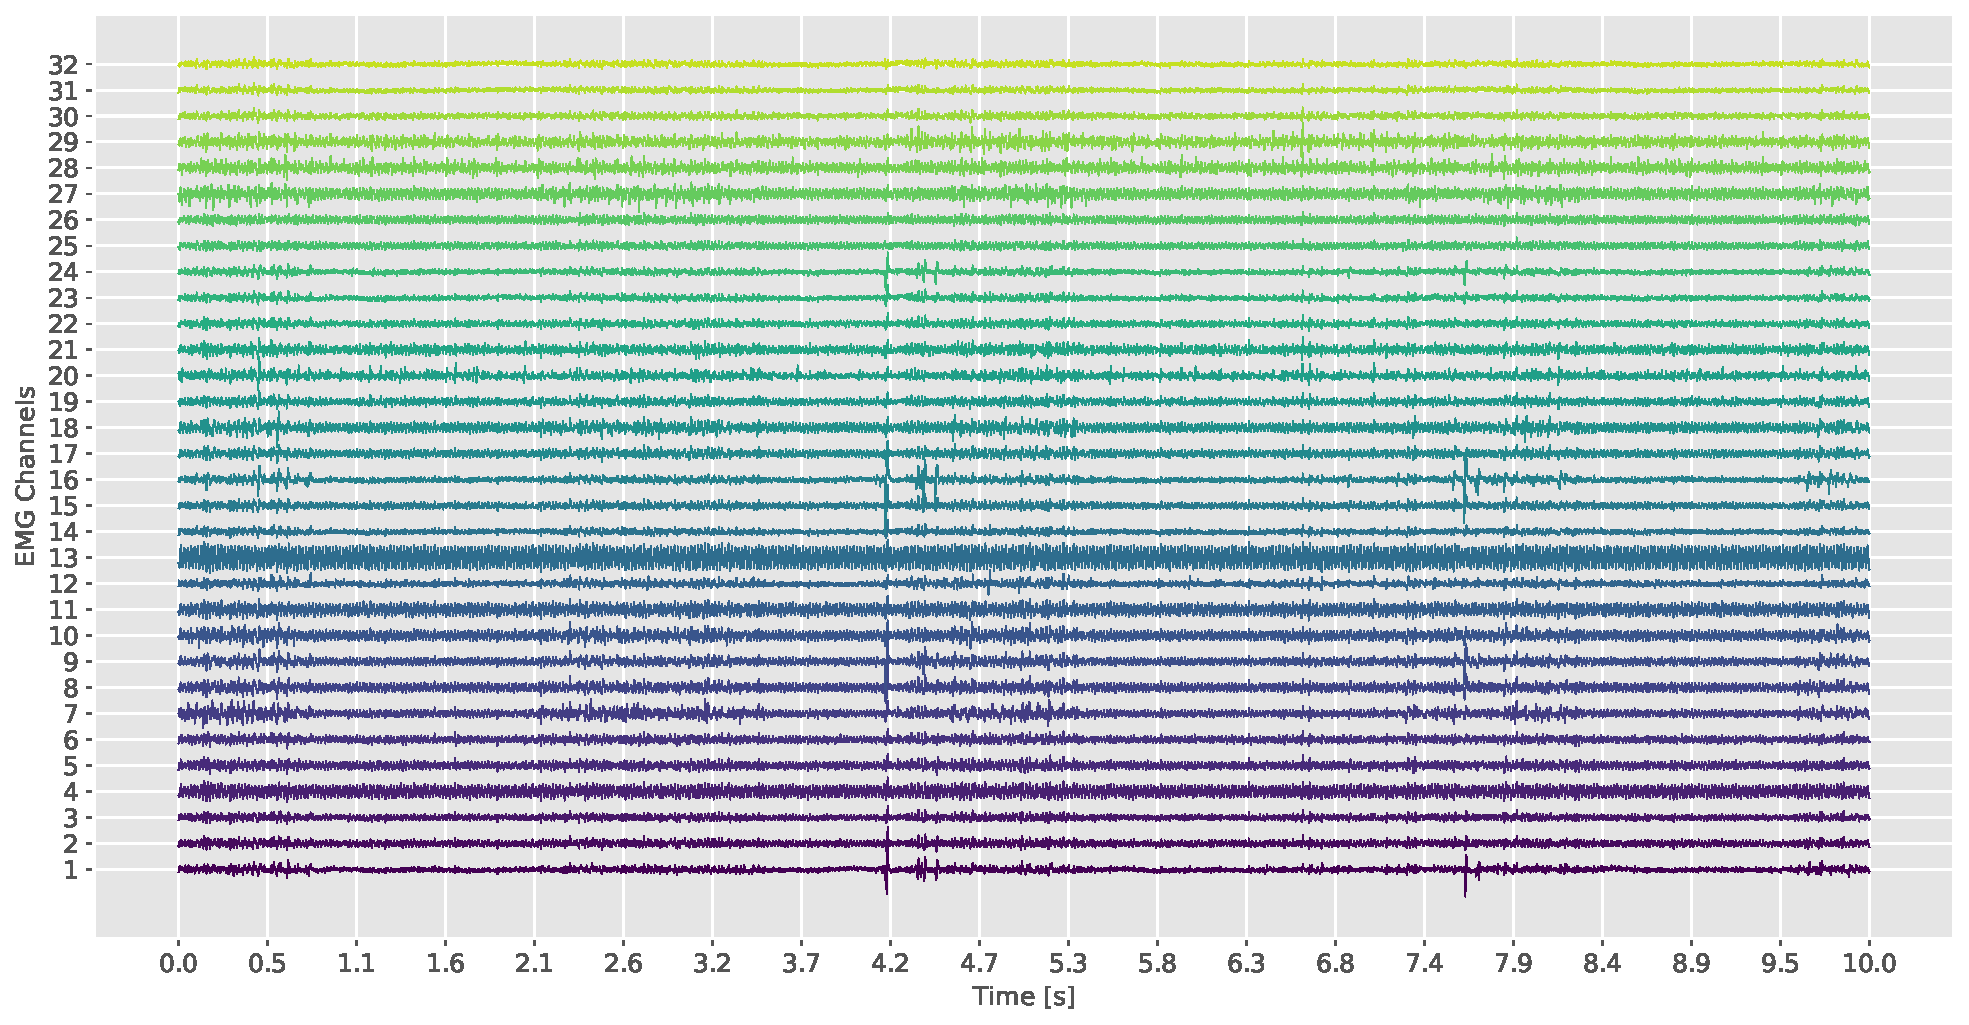
\includegraphics[width=1.0\textwidth]{methods/raw_data.pdf}
  \caption[Example raw EMG data]{10 seconds of raw 64-channel EMG data taken during a finger flexion trial. Note that some channels include some clear sine wave line noise. Putative single motor unit action potentials can be seen on many channels.}\label{fig:raw_data}
\end{figure}





\section{Task Structure}

The steps of each subject's trial:

\begin{enumerate}
  \item There are three parts of each subject's recording session: natural movement, calibration, and the target task
  \item before beginning:
  \begin{enumerate}
    \item 
    \item enter subject details, consent form sign
    \item measure arm (at ulnar styloid and 5cm below tip of elbow)
    \item choose closest sleeve size, erring on the small side, attach electrodes
    \item apply electrode paste to each electrode
    \item pre-task form fill-in (with subject metadata)
    \item clean and prep arm: soap and warm water, hard scrub
    \item place sleeve 2cm from ulnar styloid
    \item place arm in enclosure, secure hand and arm using velcro straps
    \item attach electronic ground wires to enclosure
    \item test recording: look for obvious signs of noise, electrode liftoff
    \item if issues found, adjust band, individual electrodes, or wiring
    \item explain task structure
  \end{enumerate}
  \item natural movement task:
  \begin{enumerate}
    \item ``You will be asked to perform a series of movements in the following order, \lbrack{read each movement, demonstrating each one}\rbrack. The name of each movement will appear on the screen. When the green dot appears, make this movement and hold it until the green dot disappears. The dot will last for 1 second, with a 1 second break. This will repeat three times for each movement. Try to achieve each movement to the best of your ability. Do not use your maximum force for each movement, aim for approximately 50\% of your maximum.''
    \item Answer any questions the subject may have about the task, ask if they are ready to begin
    \item Repeat this task (the series of all movements) twice 
  \end{enumerate}
  \item calibration bar task:
  \begin{enumerate}
    \item you will be asked to perform an ``exploration and isolation'' task
    \item you will see 64 vertical bars on your screen, 63 of which are white and one which is red
    \item your movements cause the bars to change in height on the screen
    \item your goal on each trial is to attempt, to the best of your ability, to maximize the height of the red bar while minimizing the height of all other bars
  \end{enumerate}
  \item fit the target task decoder:
  \begin{enumerate}
    \item run nonnegative matrix factorization with 4 components on the filtered calibration data
    \item visually inspect the modes
    \item compute the decoder, details in \Cref{sec:decoder_fitting}
    \item if an error is seen, emg is checked, calibration is repeated
    \item otherwise store the decoder and move to the target task
  \end{enumerate}
  \item target task:
  \begin{enumerate}
    \item you will be asked to move a white circular cursor from the center of the screen to a red circular targets using the muscles controlling your hand
    \item first, you must hold the cursor in the center of the screen for a required time, after which a red target will appear and the trial will begin. for the cursor to remain in the center of the screen, you must fully relax your arm and shoulder
    \item \lbrack{help the subject practice relaxing their arm, as you can hold tension in your arm and hand without realizing it. give the subject verbal instruction to help them fully relax}\rbrack
    \item if you fail to hold the cursor in the center at the start of the trial, the trial will time out and you will have three more chances to hold
    \item each trial you will attempt to hit the target with your cursor. if you are successful, a new trial will begin. if you run out of time, a new trial will begin
    \item you will attempt to complete 540 trials in total, with short breaks after each group of 180 trials
    \item after each group, I briefly interview you about any issues as needed
  \end{enumerate}
  \item \textbf{TODO} I need to explain the task spaces here more deeply, the kind of paradigm we are aiming to develop... I need a (better) figure that summarizes the linear algebra of the EMG space and the task space! I have \Cref{fig:spaces} now
  \item Each subject took about 3 hours to complete data collection 
  \end{enumerate}

  \begin{figure}[H]%[tph]
    \centering
    \includegraphics[width=1.0\textwidth]{methods/task_structure.pdf}
    \caption[Task structure for each subject]{Task structure for each subject. In the course of a session:}\label{fig:task_structure}
  \end{figure}
  



\section{Natural Movement}

\begin{itemize}
  \item purpose of this task is to establish a baseline dataset of naturalistic movements
  \item movements are individuated finger and wrist flexions and extensions, and whole-hand movements such as grasping
  \item list of movement commands shown in \Cref{fig:task_structure}
  \item No feedback is given for the subject, only movement commands
  \item Raw EMG from 64 channels recorded at 2kHz
  \item \textbf{TODO} show some stats / PCA modes / means and covariances / something else here?
\end{itemize}



\section{Calibration}

\begin{itemize}
  \item With the natural movement, we have a baseline for some typical movements subjects might make. We can use this as a proxy for naturalistic behavior
  \item If we fit a decoder to the natural movement dataset to use as a task transformation, we are likely to produce a very straightforward learning task for subjects, one that hinges on a search problem in the space of common movements rather than the wider space of possible movements (cf. \Cref{fig:spaces})
  \item The calibration task is designed to encourage exploration of the possible movement space by explicitly asking subjects to attempt to decorrelate their EMG signal channel by channel. This is the most finely grained parcellation of movements we can ask subjects to achieve though, as noted in \Cref{chap:bg_experimental}, it is known that subjects are capable of learning to control individual motor units so asking subjects to attempt channel-level control is not unreasonable.
  \item The question of this task is to what degree subjects are able to achieve channel-by-channel decorrelation of their signal
  \item Subject's success in this task, however, is not of immense importance, the critical factor is whether subjects attempt to achieve decorrelation, pushing them to explore their possible EMG space beyond the bounds of their naturalistic movement
  \item We will compare the natural movement and calibration datasets in later chapters
  \item \textbf{TODO} figure showing correlation coefficients of the target bars with the other bars-- over time, subject comparisons, etc\ldots Hypothesis: subjects are not moving randomly in this task. They are goal-oriented and are using feedback to solve this search problem. Test: compare subjects with random ``EMG'' bar heights as a null (with matching statistics)
\end{itemize}

Data processing to produce bar heights:

\begin{itemize}
  \item Starting with the raw EMG signal
  \item Highpass with a 0.1Hz cutoff using a windowed-sinc filter with a kernel width of 250 samples
  \item Rectify the signal
  \item Lowpass with a 5Hz cutoff using a windowed-sinc filter with a kernal width of 750 samples
  \item These filtering steps are common in the EMG literature (REF?) and are known to correlate will with force (REF?) when electrodes are positioned over the muscle belly
  \item Filter parameters were chosen through extensive testing with preliminary subjects who did not take part in later learning experiments
  \item See filtering steps in \Cref{fig:filtering_steps}
\end{itemize}

\begin{figure}[H]%[tph]
  \centering
  \includegraphics[width=1.0\textwidth]{methods/filtering_steps.pdf}
  \caption[Data filtering steps]{Data from a single trial showing each step of preprocessing. (TODO: finish caption.)}\label{fig:filtering_steps}
\end{figure}


\section{Target Task}


\begin{itemize}
  \item The goal of the target task is to challenge subjects with using their movements to achieve a goal
  \item Subjects' EMG signal is mapped online to a cursor shown on the screen in 2 dimensions
  \item Subjects start at rest, and when the target appears attempt for their cursor to reach the target
  \item There are 12 possible targets for each trial of the target task, spaced evenly in a unit circle. Targets appear in a randomized order
  \item The cursor is a direct, near-instantaneous mapping directly from muscle activation. The cursor is not a physics simulation of a particle with mass or friction; its position onscreen corresponds directly to the EMG signal via the computed decoder.
  \item Computation of the decoder is described in \Cref{sec:decoder_fitting}
\end{itemize}


\begin{figure}[H]%[tph]
  \centering
  \includegraphics[width=1.0\textwidth]{methods/example_trajectories.pdf}
  \caption{Cursor trajectories (blue) in two-dimensional task space during a single trial of the target task with 12 targets spaced evenly around the unit circle (active trial shown in red, non-active targets denoted by black circles, not shown to the subject in the trial). Training was conducted over 3 blocks each with 180 trials. Columns are best, median, and worst performer defined by the total hits accumulated across the target task. Rows are first, halfway, and final block of trials.}\label{fig:example_trajectories}
\end{figure}

\begin{itemize}
  \item The only additional step in the online processing of the EMG data before decoding in the target task is the standardization of the signal using the spatial (channel-wise) variance of the subject's calibration dataset. This is akin to converting EMG signal into a percentage of maximum voluntary contraction as is common in other papers. Our standardization is not a true whitening, but allows us to compare across subjects.
  \item We recorded from 46 subjects over the course of [???] weeks 
  \item Each subject's session resulted in a dataset of 
\end{itemize}


\subsection{Decoder Fitting}\label{sec:decoder_fitting}


\begin{itemize}
  \item The EMG signal is inherently nonnegative
  \item Our goal is to extract representative modes from the calibration data, directions in EMG space that capture statistics of the dataset
  \item We are not concerned with overfitting here, we just want to create a two-dimensional plane in EMG space where the likelihood that each subject's activity manifold ``covers'' or has access to the domain of the task space is high
  \item We chose Nonnegative Matrix Factorization, an unsupervised decomposition technique explained here:
\end{itemize}

Nonnegative matrix factorization (NMF) attempts to solve the following optimization:

\begin{align}
  \min{||X - WH||^{2}}
\end{align}

where $X$ is our calibration EMG data, concatenated along samples with shape $(c\times{n})$ where $N$ is the number of samples and $C$ is the number of electrode channels, fixed at 64. The objective assumes that this EMG data can be accurately reconstructed by a dot product between $W$, a $c\times{m}$ matrix which holds $m$ ``modes'', and $H$, an $m\times{n}$ matrix which holds $n$ ``activations''. For our purposes we choose \textit{a priori} to fit 4 modes, one for each cardinal direction: up, down, left, and right. The NMF process can be thought of as extracting, or inferring, an $m$-dimensional linear latent space (an $m$ dimensional plane) within the 64-dimensional EMG space. This $m$ dimensional plane, in order to reconstruct the full 64D signal, must capture the salient features of the original data.

NMF components, as they attempt to reconstruct nonnegative data, are additive. They produce components which in theory separate the input data into its constitutive parts, combined together to reform its whole.

\begin{figure}[H]%[tph]
  \centering
  \includegraphics[width=1.0\textwidth]{methods/NMF_PCA_comparison.pdf}
  \caption[Comparison of NMF and PCA]{Comparison of NMF and PCA. The leftmost plot shows a random sample fro a mixture of two 2D Gaussians (black). PCA on this data returns a simple rotation of the data aligned with the directions of maximum variance (blue arrows). The middle plot shows this data exponentiated, or lognormal. NMF is run on this data with two components and the directions which are found to maximally reconstruct this data are show (purple arrows). In the rightmost plot, we log-transform this exponentiated data (black) as well as the NMF axes (orange arrows). We also normalize these transformed axes. Thus we have a nonnegative basis for the data via NMF in both the original and lognormal spaces which reflect the dominant modes of the data, as used to generate our task decoders. This highlights the key difference between PCA and NMF\: PCA is concerned with data variance, while NMF is a ``best fit'' (up to an error tolerance) of the data's modes and does not have an immediate notion of ``explained variance''. PCA reconstructs variance, NMF reconstructs the data itself using additive components. In our task, NMF is used on the lognormal data to find modes. If comparisons are made between datasets, PCA and NMF subspaces should be compared like for like; for which this demonstration provides geometric intuition.}\label{fig:nmf_v_pca}
\end{figure}

Each NMF mode is made of up weights for each EMG channel. Once fit to a dataset, each mode can be thought of as a linear filter for each filtered EMG sample, within the original dataset or a new sample. Each filtered sample is ``projected on'' (the dot product is taken with) each mode. Thus each 64-dimensional EMG sample (a point in 64D space) is now reduced to a point in a 4D latent space, becoming an ``activation'', a linear combination of individual EMG channel readings. Mathematically, 

\begin{align}
\end{align}

where $x$ is a new sample.

\begin{align}
  X &= W\cdot{H} \\
  W^{-1}\cdot{X} &= {H}
  h_{new} = W^{-1}\cdot{x_{new}}
\end{align}

This assumes that we can compute the inverse of $W$ which in our case is rectangular. We use the Moore-Penrose pseudoinverse in place of the full inverse. Since two pairs of four modes we extract via NMF correspond to opposite directions and the mapping is linear, we subtract each pair of modes to produce a $2\times{64}$ dimensional mapping.

\begin{align}
  D &= \lbrack w_1 - w_2, w_4 - w_3 \rbrack
\end{align}

This mapping, the difference between pairs of pseudoinverse modes, is what we term the \textit{decoder.} An example of a subject's decoder is shown in \Cref{fig:example_decoder}.

\begin{itemize}
  \item \textbf{TODO} Show that we can run NMF on the second calibration dataset and compare – does similarity here correlate with performance?
\end{itemize}

\begin{figure}[H]%[tph]
  \centering
  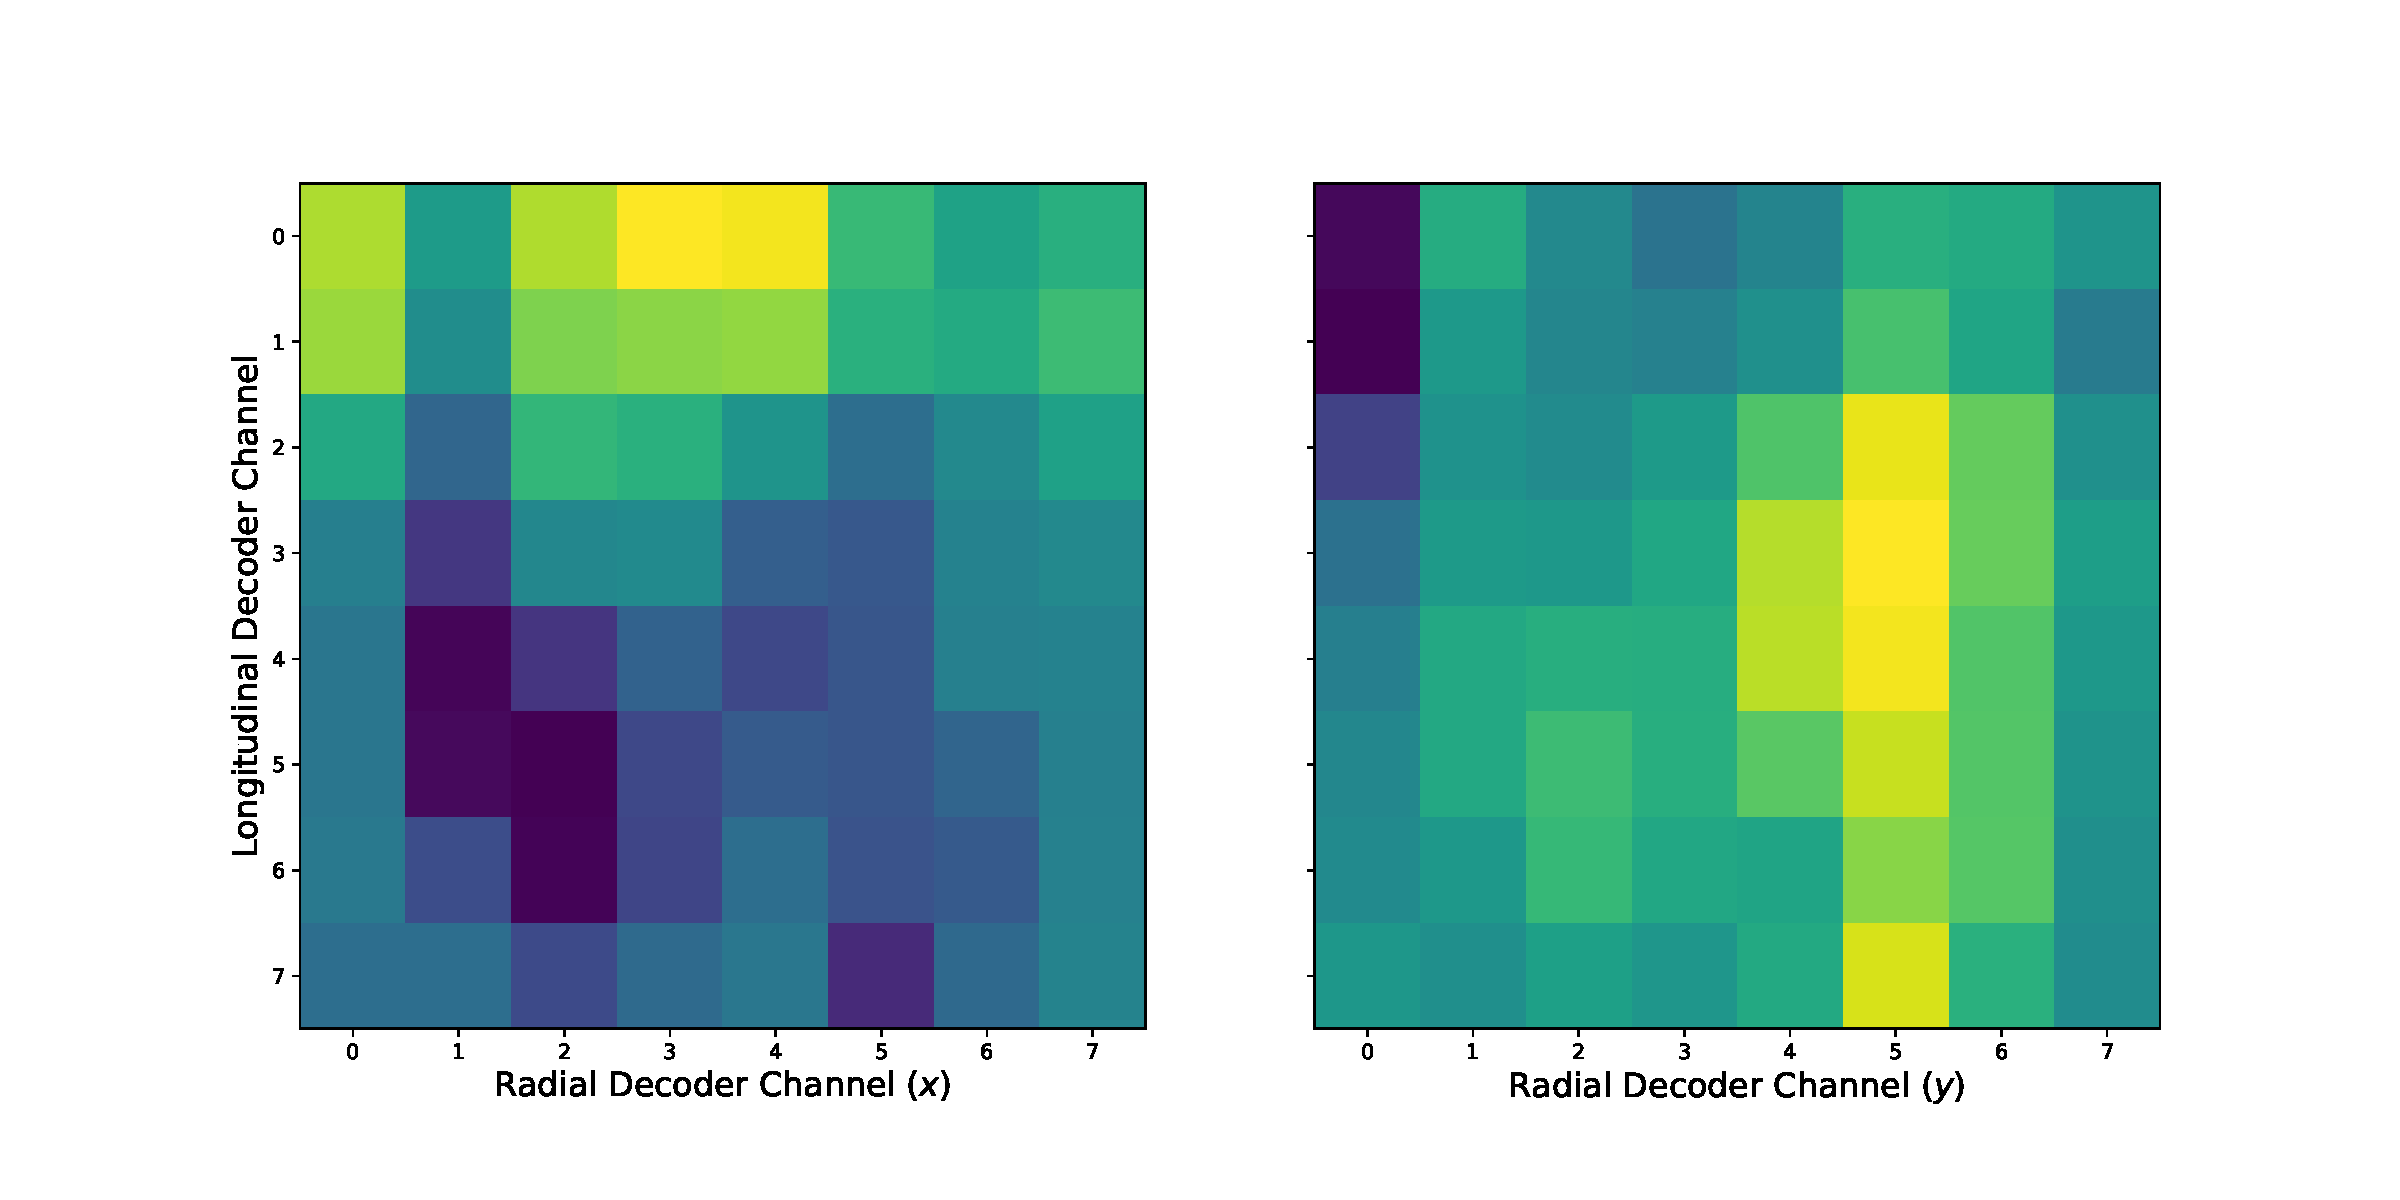
\includegraphics[width=0.7\textwidth]{methods/example_decoder.pdf}
  \caption[Example subject decoder]{Example EMG-to-cursor decoders from a single subject. The target task works by mapping 64 channels of EMG activity from subjects' forearms to 2-dimensional cursor position, a component acting in the $x$ and $y$ directions within the task's linear dynamics. Depicted here are the two 64-dimensional ``decoders'' arranged as the EMG electrodes were arranged on subjects' arms (along the arm, longitudinally, and around the arm, radially). The left plot shows the $x$ cursor decoder mode, with $y$ on the right.}\label{fig:example_decoder}
\end{figure}






\section{Offline Data Processing}

\subsection{Is the Decoder Repeatable? \lbrack{Incomplete}\rbrack}

\begin{itemize} 
  \item We used NMF to produce decoders from one of the calibration task datasets. 
  \item If we run NMF on the second calibration task dataset and compare the results to what was used in the task, are the results similar? This would confirm that the EMG space was adequately captured. 
  \item We can define a distance metric between the two decoders and test if this correlates with performance. Differences in the decoders implies that our experimental decoder did not capture the EMG space adequately enough to provide a reasonable learning challenge.
  \item \textbf{Hypothesis}: we will see similar results from the second NMF run, which will reject the hypothesis that our decoder does not well-represent subjects’ EMG movement space.
  \item \textbf{Hypothesis}: inter-decoder distance within subjects will correlate negatively with performance (different decoders, less performant). This implies that the decoder’s capturing of whole EMG space, opposed to a subspace, enables subjects to perform better on the task. We expect a crossover point here– you want an EMG search space large enough to encompass the task itself, but small enough not to provide too great of a search task for subjects.
\end{itemize}


\subsection{Is the Calibration Task Successful? \lbrack{Incomplete}\rbrack}

\begin{itemize}
  \item Compare calibration to movement in terms of variance, rank, some metric of dispersion in EMG space. \textbf{How uniformly can subjects reach their EMG space? E.g. compared to a gaussian/uniform with the same statistics?} The calibration task defines the decoder, and thus it is worth confirming that it is successful in encouraging subjects to explore their EMG space. We can compare their activity to the natural movement datasets as a baseline.
  \item Hypothesis: Variance in the calibration datasets is higher than in the natural movement dataset, even taking all natural movements together. This implies that the calibration dataset encourages exploration of a wider EMG space than that of natural movement.
\end{itemize}



\subsection{Activity Filter}

\begin{itemize}
  \item Since much of the signal is subjects at rest, we want to define and capture the ``active'' parts of EMG signal for subsequent analyses
  \item We base our activity filter on the spatial (channel-wise) 2-norm.
  \item The distribution of spatial norms appears to be lognormal, a known feature of EMG (REF?). Example histograms are shown in \Cref{fig:log_hist}
  \item Activity filter steps:
  \begin{itemize}
    \item We take the norm of the EMG samples
    \item Log transform
    \item Identify samples which are below a threshold based on the mean and standard deviation of this distribution. For the movement and calibration data, we filter out samples below half a standard deviation below the mean. For the trial data, we filter out samples below the mean. While this seems like a stringent filter, the log transformation means that we're reliably removing low activation samples to extract moments when subjects are producing goal-oriented movements.
    \item We also reject outliers, samples outside of the 1st and 99.9th percentiles.
    \item We show the result of this activity filtering in \Cref{fig:activity_filter}
  \end{itemize}
\end{itemize}


% for movement and calibration data
% log_norm = np.log(np.linalg.norm(signal,axis=1))
% mean_log_norm = np.mean(log_norm)
% std_log_norm = np.std(log_norm)
% # assuming large samples and rv being lognormal, this is roughly the 30th percentile
% mask = log_norm > (mean_log_norm - 0.5*std_log_norm)

% for trial data:
% log_norm = np.log(np.linalg.norm(signal,axis=1))
% mean_log_norm = np.mean(log_norm)
% std_log_norm = np.std(log_norm)
% # assuming large samples and rv being lognormal, this is roughly the 30th percentile
% mask = log_norm > (mean_log_norm - 0.0*std_log_norm)

% cutoffs for all data:
% samples = analysis.remove_nan_rows(subject_stack.transpose(0,1,3,2).reshape(-1,64))
% lognorms = np.log(np.linalg.norm(samples,axis=1))
% return (np.percentile(lognorms,1), np.percentile(lognorms,99.9))
% movement and calibration: 99.5
% trial: 99.9

\begin{figure}[H]%[tph]
  \begin{minipage}[b]{\linewidth}
    \centering
    \includegraphics[width=\textwidth]{methods/log_hist_movement.pdf}
    \subcaption{}
    \vspace{4ex}
  \end{minipage}\\
  \begin{minipage}[b]{\linewidth}
    \centering
    \includegraphics[width=\textwidth]{methods/log_hist_calibration.pdf}
    \subcaption{}
    \vspace{4ex}
  \end{minipage}\\
  \begin{minipage}[b]{\linewidth}
    \centering
    \includegraphics[width=\textwidth]{methods/log_hist_trial.pdf}
    \subcaption{}
    \vspace{4ex}
  \end{minipage}
  \caption[Log transforming EMG]{Activity filter!}\label{fig:log_hist}
\end{figure}

% \begin{figure}[H]%[tph]
%   \centering
%   \includegraphics[width=1.0\textwidth]{methods/activity_filter.pdf}
%   \caption[Activity filter example trial]{Activity filter!}\label{fig:activity_filter}
% \end{figure}

\begin{figure}[H]%[tph]
  \begin{minipage}[b]{0.7\linewidth}
    \centering
    \includegraphics[width=\textwidth]{methods/activity_filter_good_trial.pdf}
    \subcaption{}
    \vspace{4ex}
  \end{minipage}%%
  \begin{minipage}[b]{0.3\linewidth}
    \centering
    \includegraphics[width=\textwidth]{methods/trajectory_filter_good_trial.pdf}
    \subcaption{}
    \vspace{4ex}
  \end{minipage}
  \begin{minipage}[b]{0.7\linewidth}
    \centering
    \includegraphics[width=\textwidth]{methods/activity_filter_long_trial.pdf}
    \subcaption{}
    \vspace{4ex}
  \end{minipage}%%
  \begin{minipage}[b]{0.3\linewidth}
    \centering
    \includegraphics[width=\textwidth]{methods/trajectory_filter_long_trial.pdf}
    \subcaption{}
    \vspace{4ex}
  \end{minipage}
  \caption[Activity filter for EMG and trajectories]{Activity filter! (TODO: spruce up trajectory plots)}\label{fig:activity_filter}
\end{figure}





\cleardoublepage\printendnotes%
\ifSubfilesClassLoaded{%
    \newpage%
    \bibliography{../bib/bibliography}%
}{}%
\end{document}